%%%%%%%%%%%%%%%%%%%%%%%%%%%%%%%%%%%
%This is the LaTeX ARTICLE template for RSC journals
%Copyright The Royal Society of Chemistry 2016
%%%%%%%%%%%%%%%%%%%%%%%%%%%%%%%%%%%

\documentclass[twoside,twocolumn,9pt]{article}
\usepackage{extsizes}
\usepackage[super,sort&compress,comma]{natbib}
\usepackage[version=3]{mhchem}
\usepackage[left=1.5cm, right=1.5cm, top=1.785cm, bottom=2.0cm]{geometry}
\usepackage{balance}
\usepackage{times,mathptmx}
\usepackage{sectsty}
\usepackage{graphicx}
\usepackage{lastpage}
\usepackage[format=plain,justification=justified,singlelinecheck=false,font={stretch=1.125,small,sf},labelfont=bf,labelsep=space]{caption}
\usepackage{float}
\usepackage{fancyhdr}
\usepackage{fnpos}
\usepackage[english]{babel}
\addto{\captionsenglish}{%
  \renewcommand{\refname}{Notes and references}
}
\usepackage{array}
\usepackage{droidsans}
\usepackage{charter}
\usepackage[T1]{fontenc}
\usepackage[usenames,dvipsnames]{xcolor}
\usepackage{setspace}
\usepackage[compact]{titlesec}
\usepackage{hyperref}
\usepackage{siunitx}
%%%Please don't disable any packages in the preamble, as this may cause the template to display incorrectly.%%%


\usepackage{epstopdf}%This line makes .eps figures into .pdf - please comment out if not required.

\definecolor{cream}{RGB}{222,217,201}

\begin{document}

\pagestyle{fancy}
\thispagestyle{plain}
\fancypagestyle{plain}{

%%%HEADER%%%
\fancyhead[C]{\includegraphics[width=18.5cm]{head_foot/header_bar}}
\fancyhead[L]{\hspace{0cm}\vspace{1.5cm}\includegraphics[height=30pt]{head_foot/journal_name}}
\fancyhead[R]{\hspace{0cm}\vspace{1.7cm}\includegraphics[height=55pt]{head_foot/RSC_LOGO_CMYK}}
\renewcommand{\headrulewidth}{0pt}
}
%%%END OF HEADER%%%

%%%PAGE SETUP - Please do not change any commands within this section%%%
\makeFNbottom
\makeatletter
\renewcommand\LARGE{\@setfontsize\LARGE{15pt}{17}}
\renewcommand\Large{\@setfontsize\Large{12pt}{14}}
\renewcommand\large{\@setfontsize\large{10pt}{12}}
\renewcommand\footnotesize{\@setfontsize\footnotesize{7pt}{10}}
\makeatother

\renewcommand{\thefootnote}{\fnsymbol{footnote}}
\renewcommand\footnoterule{\vspace*{1pt}%
\color{cream}\hrule width 3.5in height 0.4pt \color{black}\vspace*{5pt}}
\setcounter{secnumdepth}{5}

\makeatletter
\renewcommand\@biblabel[1]{#1}
\renewcommand\@makefntext[1]%
{\noindent\makebox[0pt][r]{\@thefnmark\,}#1}
\makeatother
\renewcommand{\figurename}{\small{Fig.}~}
\sectionfont{\sffamily\Large}
\subsectionfont{\normalsize}
\subsubsectionfont{\bf}
\setstretch{1.125} %In particular, please do not alter this line.
\setlength{\skip\footins}{0.8cm}
\setlength{\footnotesep}{0.25cm}
\setlength{\jot}{10pt}
\titlespacing*{\section}{0pt}{4pt}{4pt}
\titlespacing*{\subsection}{0pt}{15pt}{1pt}
%%%END OF PAGE SETUP%%%

%%%FOOTER%%%
\fancyfoot{}
\fancyfoot[LO,RE]{\vspace{-7.1pt}\includegraphics[height=9pt]{head_foot/LF}}
\fancyfoot[CO]{\vspace{-7.1pt}\hspace{13.2cm}\includegraphics{head_foot/RF}}
\fancyfoot[CE]{\vspace{-7.2pt}\hspace{-14.2cm}\includegraphics{head_foot/RF}}
\fancyfoot[RO]{\footnotesize{\sffamily{1--\pageref{LastPage} ~\textbar  \hspace{2pt}\thepage}}}
\fancyfoot[LE]{\footnotesize{\sffamily{\thepage~\textbar\hspace{3.45cm} 1--\pageref{LastPage}}}}
\fancyhead{}
\renewcommand{\headrulewidth}{0pt}
\renewcommand{\footrulewidth}{0pt}
\setlength{\arrayrulewidth}{1pt}
\setlength{\columnsep}{6.5mm}
\setlength\bibsep{1pt}
%%%END OF FOOTER%%%

%%%FIGURE SETUP - please do not change any commands within this section%%%
\makeatletter
\newlength{\figrulesep}
\setlength{\figrulesep}{0.5\textfloatsep}

\newcommand{\topfigrule}{\vspace*{-1pt}%
\noindent{\color{cream}\rule[-\figrulesep]{\columnwidth}{1.5pt}} }

\newcommand{\botfigrule}{\vspace*{-2pt}%
\noindent{\color{cream}\rule[\figrulesep]{\columnwidth}{1.5pt}} }

\newcommand{\dblfigrule}{\vspace*{-1pt}%
\noindent{\color{cream}\rule[-\figrulesep]{\textwidth}{1.5pt}} }

\makeatother
%%%END OF FIGURE SETUP%%%

%%%TITLE, AUTHORS AND ABSTRACT%%%
\twocolumn[
  \begin{@twocolumnfalse}
\vspace{3cm}
\sffamily
\begin{tabular}{m{4.5cm} p{13.5cm} }

\includegraphics{head_foot/DOI} & \noindent\LARGE{\textbf{Applying molecular simulation to the analysis of lipid monolayer reflectometry$^\dag$}} \\%Article title goes here instead of the text "This is the title"
\vspace{0.3cm} & \vspace{0.3cm} \\

 & \noindent\large{Andrew R. McCluskey,$^{\ast}$\textit{$^{a,b}$} James Grant,\textit{$^{c}$} Andrew J. Smith,\textit{$^{b}$} Jonathan L. Rawle,\textit{$^{b}$} David J. Barlow,\textit{$^{d}$} M. Jayne Lawrence,\textit{$^{e}$} Stephen C. Parker,\textit{$^{a}$} and Karen J. Edler$^{\ast}$\textit{$^{a}$}} \\%Author names go here instead of "Full name", etc.

\includegraphics{head_foot/dates} & \noindent\normalsize{The abstract should be a single paragraph which summarises the content of the article. Any references in the abstract should be written out in full \textit{e.g.}\ [Surname \textit{et al., Journal Title}, 2000, \textbf{35}, 3523].} \\%The abstrast goes here instead of the text "The abstract should be..."

\end{tabular}

 \end{@twocolumnfalse} \vspace{0.6cm}

  ]
%%%END OF TITLE, AUTHORS AND ABSTRACT%%%

%%%FONT SETUP - please do not change any commands within this section
\renewcommand*\rmdefault{bch}\normalfont\upshape
\rmfamily
\section*{}
\vspace{-1cm}


%%%FOOTNOTES%%%

\footnotetext{\textit{$^{a}$~Department of Chemistry, University of Bath, Claverton Down, Bath, BA2 7AY, UK. E-mail: a.r.mccluskey@bath.ac.uk/k.edler@bath.ac.uk}}
\footnotetext{\textit{$^{b}$~Dimaond Light Source, Diamond House, Rutherford Appleton Laboratory, Harwell Oxford, OX11 0DE, UK.}}
\footnotetext{\textit{$^{c}$~Computing Services, University of Bath, Claverton Down, Bath, BA2 7AY, UK.}}
\footnotetext{\textit{$^{d}$~Institute of Pharmaceutical Science, King's College London, London, SE1 9NH, UK.}}
\footnotetext{\textit{$^{e}$~Division of Pharmacy and Optometry, University of Manchester, Manchester, M13 9PT, UK.}}

%Please use \dag to cite the ESI in the main text of the article.
%If you article does not have ESI please remove the the \dag symbol from the title and the footnotetext below.
\footnotetext{\dag~Electronic Supplementary Information (ESI) available: All analysis/plotting scripts and figure files, allowing for a fully reproducible and automated workflow for the work presented is available at \url{https://github.com/arm61/simulation_vs_traditional_reflectometry} (DOI: 10.xxxx/xxxxxxxx/)}
%additional addresses can be cited as above using the lower-case letters, c, d, e... If all authors are from the same address, no letter is required

%\footnotetext{\ddag~Additional footnotes to the title and authors can be included \textit{e.g.}\ `Present address:' or `These authors contributed equally to this work' as above using the symbols: \ddag, \textsection, and \P. Please place the appropriate symbol next to the author's name and include a \texttt{\textbackslash footnotetext} entry in the the correct place in the list.}


%%%END OF FOOTNOTES%%%

%%%MAIN TEXT%%%%
\section{Introduction}
Neutron and X-ray reflectometry techniques are popular in the study of nanolayered structures, such as surfactant monolayers,\cite{Hazell2016} lipid bilayer systems,\cite{Belicka2015} nanoparticle films,\cite{Velleman2016} and dye-sensitised solar cell materials.\cite{McCreeGrey2015}
Unlike other surface-sensitive techniques, such as atomic force microscopy (AFM) or scanning electron microscopy (SEM), reflectometry techniques are able to investigate buried interfaces in addition to the material surface.
This is due to the fact that neutrons and X-rays can probe more deeply into a material than an AFM tip or the electron.
Additionally, reflectometry techniques can more easily provide information about the average structure of a material due to the nature of measuring over large regions of space, resulting in significantly improved sampling, compared with microscopy techniques.\cite{Renaud2009}

The growth in popularity of reflectometry techniques can be attributed to the significant development of reflectometry instrumentation, such as FIGARO, the horizontal neutron reflectometer at the ILL,\cite{Campbell2011} and the beam deflection system at the I07 beamline of the Diamond Light Source.\cite{Arnold2012}
These developments have enabled the study of more complex systems including bacterial membrane,\cite{Barker2016} and polymeric energy materials.\cite{Khodakarimi2016}
However, the ability to study complex systems poses an important data analysis challange, where traditional methods may not be sufficient.

The Abel\`{e}s matrix formalism for stratified media, \cite{Abeles1950} is the most commonly applied method to analyse reflectometry data from a surfactant monolayer.
This method involves the construction of a layer model of the system under study, the calculation of the reflectometry from such a system and the refinement of this model with respect to the experimental reflectometry data.
This has been used to study surfactant self-assembly at the air-liquid interfaces in single and double tailed sulfobetaine lipids,\cite{Hazell2016} showing the monolayer structure of these novel lipids to be simuilar to that observed for traditional lipid molecules.
It has also being applied to the anlaysis of a supported lipid bilayer by Hellstrand \emph{et al.}\cite{Hellstrand2013} where it allowed for the observation of the adsorption of the protein $\alpha$-synnuclein, which was found to reside in the head-group region of the bilayer.

The Abel\`{e}s matrix formalism is often described as the dynamical approach to reflectometry analysis, in contrast to the Fourier transform-based kinematic approach.\cite{Crowley1991,Lu1996}
The dynamical approach considers the reflection and refraction of the probing radiation at a series of interfaces, where the refractive index is a function of the scattering length densities (SLDs) for each layer.
By considering Figure \ref{fig:dyn} it is clear how the reflected radiation could interact coherently and incoherently in analogy with Bragg's law.
%
\begin{figure}[h]
\centering
  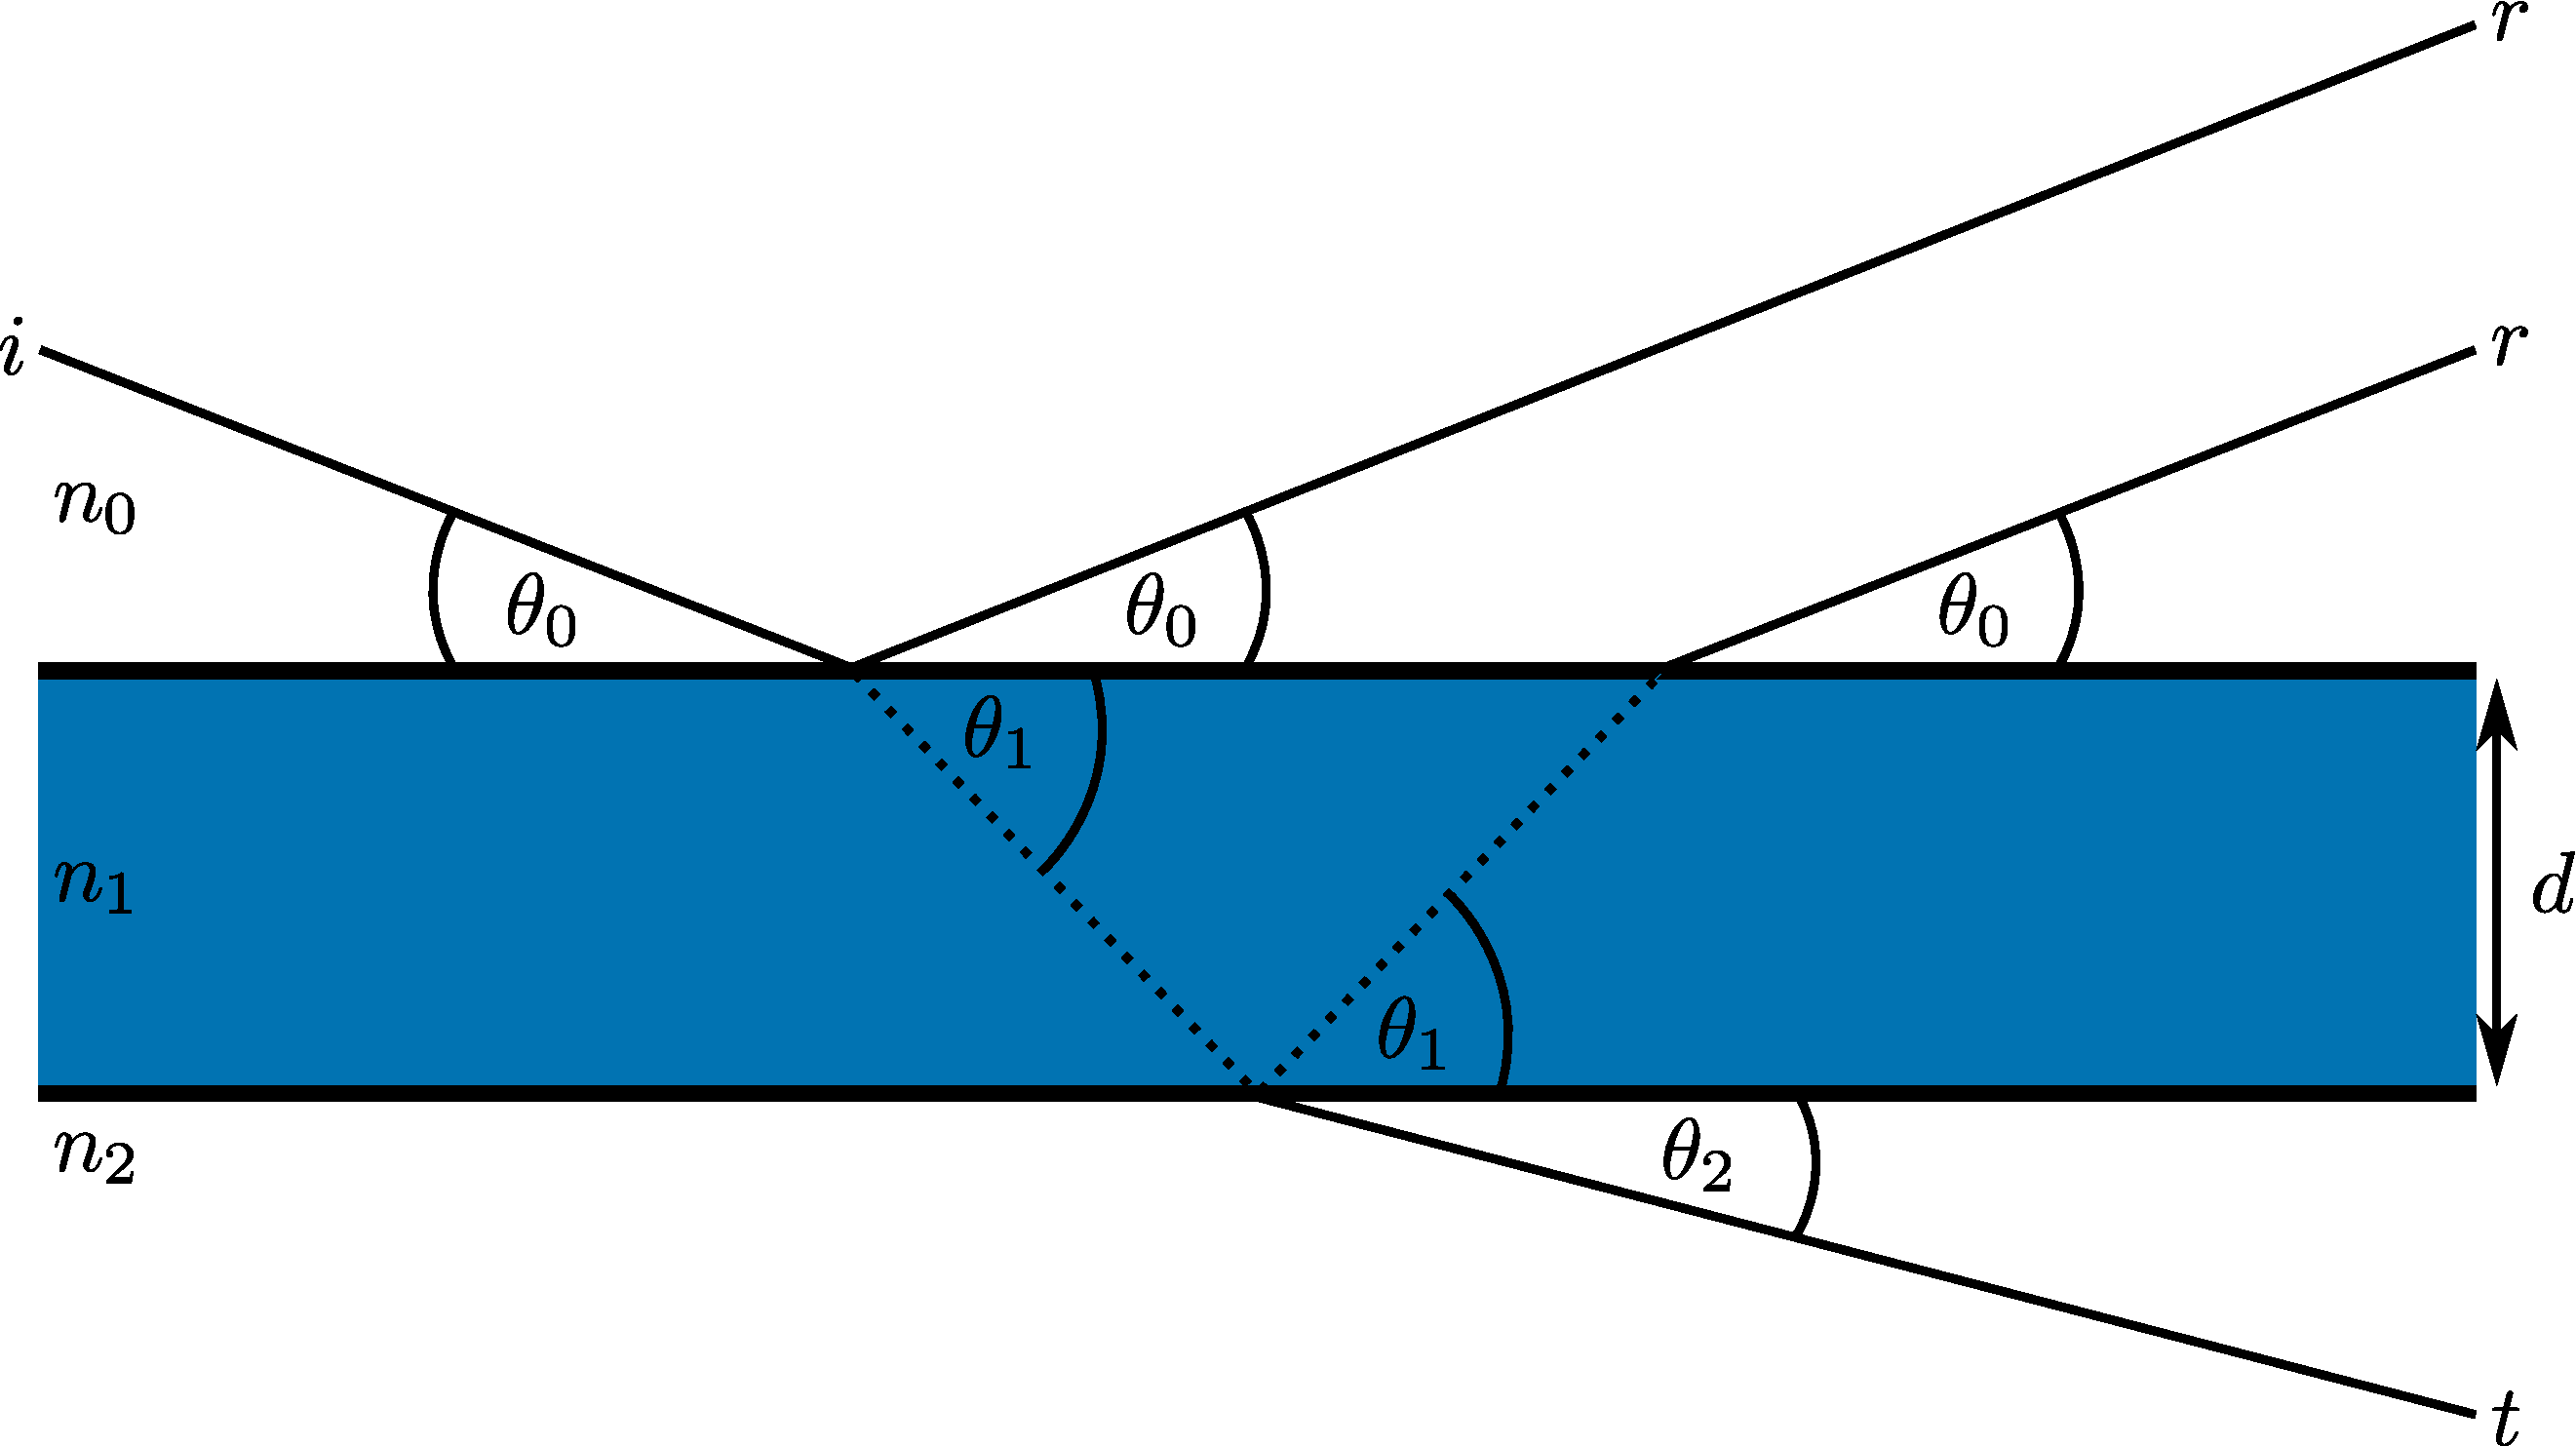
\includegraphics[width=0.48\textwidth]{figures/reflrefr}
  \caption{A schematic of a reflectometry experiment, where $i$ is the incident radiation, $r$ is the reflected radiation, $t$ is the transmitted radiation, and $d$ is the layer thickness, for each layer $n$.}
  \label{fig:dyn}
\end{figure}
%

A commonly suggested method for the multi-modal analysis of reflectometry measurements is the use of molecular dynamics (MD) simulations.
This has been applied previously, either by the calculation of the SLD profile from the simulation or the full determination of the reflectometry profile.
In the former case, the calculated SLD profile may be compared with the SLD profile determined from the use of a traditional analysis method.
Bobone \emph{et al.} used such a method to study the antimicrobial peptide trichogin GA-IV within a supported lipid bilayer.\cite{Bobone2013}
A four layer model consisting of the hydrated \ce{SiO2} layer, an inner lipid head-region, a lipid tail-region, and an outer lipid head region was used in the Abel\`{e}s matrix formalism.
The SLD profile from the MD simulations agreed well with that fitted to the reflectometry data from the layer model.

The reflectometry profile was calculated explicitly from classical simulation in the works of Miller \emph{et al.} and Anderson and Wilson.\cite{Miller2003,Anderson2004}
In these, an amphiphilic polymer at the oil-water interface was simulated by Monte Carlo and MD respectively, and the neutron reflectometry profile for found by splitting the simulation cell into a series of small layers and applying the Abel\`{e}s matrix formalism.
There was good agreement between the experimental and calculated reflectometry, for low interface coverages of the polymer.
Another work that has made direct comparison between the atomistic simulation-derived reflectometry and those measured experimentally includes that of Darr\'{e} \emph{et al.}.\cite{Darre2015}
In this work, NeutronRefTools was developed to produce the neutron reflectometry profile from a given MD simulation.
The particular system studied was a supported DMPC lipid bilayer, with some agreement found between the simulation-derived profile and the experimental measurement.
However, the nature of the support required a correction for the head-group hydration to be imposed to achieve a good fit to the data.

Koutsioubas used the MARTINI coarse-grained representation of a DPPC lipid bilayer to compare with experimental reflectometry.\cite{Koutsioubas2016}
This work shows that the parameterisation of the MARTINI water bead was extremely important in the reporduction of the reflectometry data, as the non-polarisable water bead would freeze into crystalline sheets resulting in artefacts in the reflectometry profiles calculated.
Finally, the work of Hughes \emph{et al.} again studied a DPPC lipid bilayer system,\cite{Hughes2016} albeit an all-atom representation, that was compared with a supported DPPC lipid bilayer system measured with polarised neutron reflectometry.
The SLD profile found from MD was varied to fit better with the experimental measurement, resulting in good agreement.
Additionally, the variation of the SLD profile was used to remove artifacts that arose from poor splicing between the MD simulations that the layer model used in regions such as the gold and magnetic permalloy layers not present in the simulation.

In all of the examples discussed, there is no direct comparison between the reflectometry profile determined from simulation and that from the application of a traditional analysis method.
Herein, we present the first, to the authors knowledge, example of such a comparison, wherein three different MD simulation force-fields of various particle grain-size have been considered; namely the Slipid all-atom,\cite{Jambeck2012} Berger united-atom,\cite{Berger1997} and MARTINI coarse-grained force fields.\cite{Marrink2007}
We believe that this work provides bath a fundemental insight into the validity and utility of using simulation-derived analysis for reflecometry measurements, as well as offering an important discussion of the utility of coarse-grained simulation within such a framework.

\section{Methodology}

\subsection{Neutron reflectometry measurements}
The neutron reflectometry measurements analysed in this work have been previously published by Hollinshead \emph{et al.},\cite{Hollinshead2009} and full details of the methods used can be found in this previous publication.
These measurements involves studying seven contrasts of 1,2-distearoyl-\emph{sn}-phosphatidylcholine (DSPC) at the air-water interface (Table \ref{tbl:nom}), at four different surface pressures; \SIrange{20}{50}{\milli\newton\per\meter}.
%
\begin{table}[h]
\small
  \caption{\ The different contrasts of lipid and water investigated in this work. ACMW is air-contrast matched water, where \ce{D2O} and \ce{H2O} are mixed such as to given a water with a SLD of zero.}
  \label{tbl:nom}
  \begin{tabular*}{0.48\textwidth}{@{\extracolsep{\fill}}lll}
    \hline
    Shorthand & Lipid contrast & Water contrast \\
    \hline
    h-\ce{D2O} & h-DSPC & \ce{D2O} \\
    \ce{d_{13}}-ACMW & \ce{d_{13}}-DSPC & ACMW \\
    \ce{d_{13}}-\ce{D2O} & \ce{d_{13}}-DSPC & \ce{D2O} \\
    \ce{d_{70}}-ACMW & \ce{d_{70}}-DSPC & ACMW \\
    \ce{d_{70}}-\ce{D2O} & \ce{d_{70}}-DSPC & \ce{D2O} \\
    \ce{d_{83}}-ACMW & \ce{d_{83}}-DSPC & ACMW \\
    \ce{d_{83}}-\ce{D2O} & \ce{d_{83}}-DSPC & \ce{D2O} \\
    \hline
  \end{tabular*}
\end{table}
%

\subsection{Molecular dynamics simulations}
The DSPC monolayer simulation were made up of lipid molecules modelled with three force-fields, each of a different particles grain-size.
The Slipids force-field is an all-atom representation of the lipid molecules,\cite{Jambeck2012} which was used alongside the single point charge (SPC) water model,\cite{Berendsen1987} with a leap-frog integrator and a timestep of \SI{0.5}{\femto\second}.
The Berger force-field is obtained by integrating out the hydrogen atoms to produce a united atom force-field,\cite{Berger1997} again the leap-frog integrator and SPC water molecules were used.
The removal of the high frequency \ce{C-H} bonds allows fo the timestep to be increased to \SI{1}{\femto\second}.
Finally, the lowest resolution force-field that was used was the MARTINI\cite{Marrink2007} alongside the polarisable MARTINI water model,\cite{Yesylevskyy2010} to avoid the freezing issues observed previously.\cite{Koutsioubas2016}
The MARTINI 4-to-1 heavy atom beading allows for the use of a \SI{20}{\femto\second} timestep to be used, again with a leap-frog integrator.
All simulations were conducted with a temperature coupling to a heat bath at \SI{300}{\kelvin}, and run using GROMACS 5.0.5 \cite{Berendsen1995,Lindahl2001,vanderSpoel2005,Hess2008} on 32 cores of the STFC Scientific Computing resource SCARF.
The simulation was of a monolayer, therefore the Ewald 3DC correction was applied to allow for the use of \emph{x}/\emph{y}-only periodic boundary conditions.\cite{InChul1999}
A ``wall'' of non-interacting dummy atoms was placed at each side of the simulation cell in the \emph{z}-direction to ensure that the atoms would not pass out of the simulation cell.

The starting simulation structure was generated using the molecular packing software Packmol.\cite{Martinez2009}
This was used to produce a monolayer of 100 DSPC molecules, with the head group oriented to the bottom of the simulation cell.
A \SI{6}{\angstrom} layer of water was then added such that the head groups were overlapping, this was achieved using the \texttt{solvate} functionality in GROMACS 5.0.5.
Examples of the dry and wet monolayer can be seen in Figure \ref{fig:drywet} for the Berger force-field system.
A general protocal was then used to relax the system at the desired surface coverage, reproducing the effects of a Langmuir trough \emph{in-silico}.
This involved subjecting the system to a semi-isotropic barosts, with a compressibility of \SI{4.5E-5}{\per\bar} of the Slipids and Berger simulations and \SI{3.0E-4}{\per\bar} for the MARTINI simulations.
The pressure in the \emph{z}-dimension was kept constant at \SI{1}{\bar}, while it was increased in the \emph{x}- and \emph{y}-dimensions isotropically.
When the \emph{xy}-surface area is reached that is associated with the area per molecule (APM) for each surface pressure, described by the experimental surface pressure-isotherm (Figure \ref{fig:iso}), given in Table \ref{tbl:apm}, the coordinates were save and used as the starting structure for the equilibration simulation.
This involves continuing the use of the semi-isotropic barostat, with the \emph{xy}-area of the box fixed.
This allowed the system to relax at a pressure of \SI{1}{\bar} in the \emph{z}-dimension.
The equilibration period was \SI{1}{\nano\second}, following which the \SI{50}{\nano\second} NVT ensemble production simulations were run, on which all analyses were conducted.
%
\begin{figure}[h]
\centering
  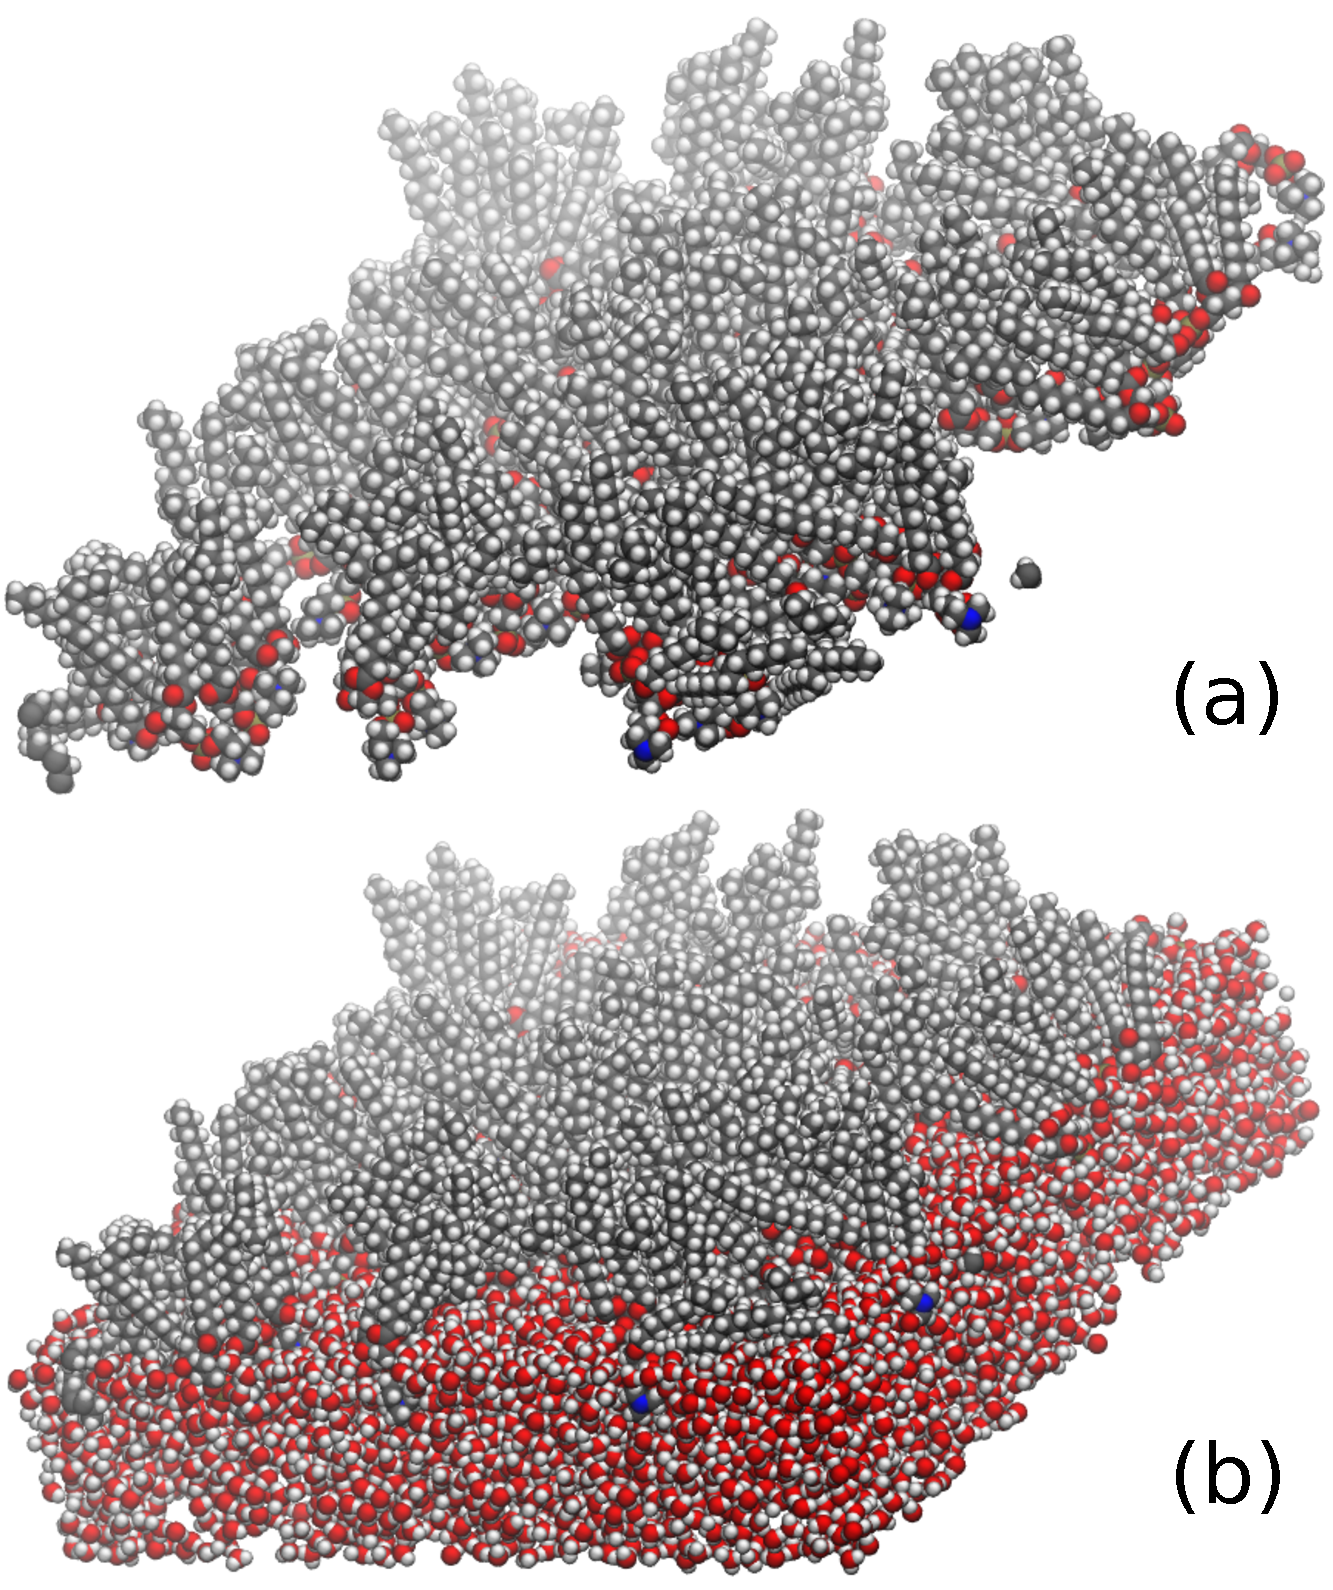
\includegraphics[width=0.4\textwidth]{figures/dspcdrywet}
  \caption{The DSPC monolayer (a) without water layer and (b) with water layer, visuallised using VMD.\cite{Humphrey1996}}
  \label{fig:drywet}
\end{figure}
%
%
\begin{figure}[h]
\centering
  \includegraphics[width=0.48\textwidth]{figures/apm}
  \caption{The experimental surface pressure isotherm for DSPC, taken from the work of Kubo \emph{et al.}\cite{Kubo2001}}
  \label{fig:iso}
\end{figure}
%
%
\begin{table}[h]
\small
  \caption{\ The areas per molecule (APM) associated with particular surface pressures and the size of the \emph{x}- and \emph{y}-cell dimension for a simulation of 100 lipid molecules.}
  \label{tbl:apm}
  \begin{tabular*}{0.48\textwidth}{@{\extracolsep{\fill}}lll}
    \hline
    $\pi$/\si{\milli\newton\per\meter} & APM/\si{\per\angstrom\squared} & \emph{xy}-cell length/\si{\angstrom} \\
    \hline
    20 & 47.90 & 69.07 \\
    30 & 46.40 & 68.12 \\
    40 & 45.00 & 67.08 \\
    50 & 44.58 & 66.01 \\
    \hline
  \end{tabular*}
\end{table}
%

\subsection{Abel\`{e}s matrix formalism}
To compare against the simulation-derived reflectometry profiles, the chemically-consistant surfactant monolayer model was used.\cite{McCluskey2018,McCluskey2018a}
This model is implemented as a class that is compatible with the Python package refnx.\cite{Nelson2018,refnx}
The model is made up of two layer; the head-layer at the interface with the solvent and the tail-layer at the interface with the air.
The head components have a calculated scattering length, $b_h$, (found as a summation of the neutron scattering lengths of the individual atoms) and a component volume, $V_h$.
These make up a head-layer with a given thickness, $d_h$, and interfacial roughness, $\sigma_h$, within this layer some volume fraction of solvent may intercalate, $\phi_h$.
The tail components also have a similarly calculated scattering length, $b_t$, and component volume, $V_t$.
In this work, the length of the hydrocarbon tail, $t_t$, as defined by the Tanford Equation,\cite{Tanford1980}
%
\begin{equation}
  t_t = 1.54 + 1.265n,
\end{equation}
%
where $n$ is the number of carbon atoms in the chain, therefore for DSPC $t_t = \SI{24.3}{\angstrom}$.
The tail-layer thickness is then found by considering $t_t$ and the angle that the chain is tilted by with respect to the interface normal, $\theta_t$,
%
\begin{equation}
  d_t = t_t\cos{\theta_t}.
\end{equation}
%
This was used to impose a chemically-sensible maximum on the thickenss of the tail-layer, e.g. it cannot be thicker than the maximum extended tail length of the lipid.
The SLD of the tail and head layers used in the Abel\`{e}s matrix formalism can therefore be found as,
%
\begin{equation}
  \text{SLD}_i = \frac{b_i}{V_i}(1 - \phi_i) + \text{SLD}_s(\phi_i),
\end{equation}
%
where, $\text{SLD}_s$ is the scattering length density of the subphase (water), and $i$ indicates either the tail- or head-layer; it is assumed that the tail layer contains no solvent or air, e.g. $\phi_t = 0$.
To ensure that the number density of the head components and pairs of tail components is the same, the following constraint was included in the model,\cite{Braun2017}
%
\begin{equation}
  \phi_h = 1 - \bigg(\frac{d_tV_h}{V_td_h}\bigg).
\end{equation}
%
Based on the work of Campbell \emph{et al.},\cite{Campbell2018} a single value for the interfacial roughness was fit for all interfaces, as there is only a single lipid type in each monolayer.
Therefore, any capillary wave roughness at the air-water interface is carried equally through all the layers.
The only modification made to this monolayer model used previous was that the tail component volume was also constrained, based on the APM (taken from the surface pressure isotherm),
%
\begin{equation}
  V_t = d_t \text{APM}.
\end{equation}
%
The result of this is that both the monolayer model and the simulation-derived models were constrained equally by this calculated surface coverage.

In this work, the experimental data from all seven contrasts were co-refined to a single monolayer model, where the head thickness, chain tilt angle, head component volume, and interfacial roughness were allowed to vary.
The values of the head and tail scattering lengths, along with the super and subphase SLDs are given in Table S1.
The length of the tail chain was kept constant at \SI{24.3}{\angstrom}, as defined by the Tanford equation.\cite{Tanford1980}
This is due to the monolayer being investigated at relatively high surface pressures, where the extended, staggered conformation is likely to be present.
For each co-refinement of seven neutron reflectometry measurements, there were in total five degrees of freedom in the fitting process.

\subsection{Simulation-derived analysis}
Version 1.0.1 of refnx\cite{Nelson2018,refnx} includes the ability to obtain simulation-derived reflectometry profiles, using a similar method to that employed in previous work, such as Darr\'{e} \emph{et al.}.\cite{Darre2015}
The Abel\`{e}s matrix formalism is applied on layers, the SLD of which is drawn directly from the simulation, and the thickness of which is defined.
The interfacial roughness between these layers is defined as \SI{0}{\angstrom} for the Slipid and Berger force-field simulations.
However a value of \SI{0.8}{\angstrom} was used in the MARTINI force-field simulations, a detailed discussion for the rationale behind this is available in the ESI.
Each of the \SI{50}{\nano\second} production simulations were analysed with a frequency of every \SI{0.1}{\nano\second}, and the SLD profiles were determined by summing the scattering lengths, $b_j$, for each of the atoms in a given layer.
%
\begin{equation}
  \text{SLD}_n = \frac{\sum_j{b_j}}{V_n},
\end{equation}
%
where, $V_n$ is the volume of the layer $n$, obtained from the simulation cell parameters in the plane of the interface and the defined layer thickness.
A uniform background and scale factor was then determined using refnx to offer the best agreement between the calculated reflectometry profile and that determined experimentally.

\subsection{Comparison between monolayer model and simulation-derived analysis}
\label{sec:para}
In order to assess the agreement between the models from each method, the following goodness-of-fit metric was used, following the transformation of the data into $Rq^4$ space,
%
\begin{equation}
  \chi^2 = \sum_{i=1}^{N_{\text{data}}} \frac{[R_{\text{exp}}(q_i) - R_{\text{sim}}(q_i)]^2}{[\delta R_{\text{exp}}(q_i)]^2},
\end{equation}
%
where $q_i$ is a given $q$-vector, $R_{\text{exp}}(q_i)$ is the experimental reflected intensity, $R_{\text{sim}}(q_i)$ is the simulation-derived reflected intensity, and $\delta R_{\text{exp}}(q_i)$ is the resolution function of the data.

Parameterical outcomes from the different analysis methods were also compared, such as the number of water molecules per head group, wph.
This was obtained from the monolayer model by considering the solvent fraction in the head-layer, $\phi_h$, the volume of the head group, $V_h$, and taking the volume of a single water molecule to be \SI{29.9}{\cubic\angstrom},
%
%\begin{equation}
%  \text{wph} = \frac{\phi_hV_h}{29.9 - 29.9\phi_h}.
%\end{equation}
%
From the molecular dynamics simulation, the number densities for each component of the system were determined.
The ratio of the integrals of the lipid heads and the water then gave the wph.
The range for this integral was taken as between the \SI{5}{\percent} and \SI{95}{\percent} quantiles of the lipid head-layers.

It was also possible to compare the tilt of the lipid tails with respect to the surface normal.
This angle was used as a fitting parameter in the monolayer model, and can be obtained directly from the MD simulation.
For this, a vector was defined between the first and last carbon atoms of each chain and the angle with respect to the surface normal was found trigonometrically.

\section{Results \& Discussion}

\subsection{Comparison between models}
%
\begin{figure*}
 \centering
 \includegraphics[width=0.49\textwidth]{figures/trad_30}
 \includegraphics[width=0.49\textwidth]{figures/sim_slipids_30} \\
 \includegraphics[width=0.49\textwidth]{figures/sim_berger_30}
 \includegraphics[width=0.49\textwidth]{figures/sim_martini_30}
 \caption{A comparison of the reflectometry and SLD profiles obtained from (a) the monolayer model, (b) the Slipid simulation, (c) the Berger force-force simulation, and (d) the MARTINI force-field simulation at a surface pressure of \SI{30}{\milli\newton\per\meter}. From top-to-bottom the contrasts are as follows; \ce{d_{83}}-\ce{D2O}, \ce{d_{83}}-ACMW, \ce{d_{70}}-\ce{D2O}, \ce{d_{70}}-ACMW, h-\ce{D2O}, \ce{d_{13}}-\ce{D2O}, \ce{d_{13}}-ACMW. The different contrast reflectometry profiles have been offset in the \emph{y}-axis by an order of magnitude and the SLD profiles offset in the \emph{y}-axis by \SI{1e-6}{\per\square\angstrom}, for clarity.}
 \label{fig:ref}
\end{figure*}
%
Figure \ref{fig:ref} compares the reflectometry and SLD profiles from each of the different methods used at a surface pressure of \SI{30}{\milli\newton\per\meter}.
The data for the other surface pressures showed similar trends, and can be found in the ESI.
The $\chi^2$ goodness-of-fit metric between the calculated and experimental reflectometry is given in Table \ref{tbl:chi} for each contrast, in addition to a sum of all contrasts.
%
\begin{table*}
\small
  \caption{\ The goodness-of-fit between the calculated and experimental reflectometry profile at a surface pressure of \SI{30}{\milli\newton\per\metre}.}
  \label{tbl:chi}
  \begin{tabular*}{\textwidth}{@{\extracolsep{\fill}}lllll}
    \hline
    Contrast & Monolayer model & Slipid & Berger & MARTINI \\
    \hline
    h-\ce{D2O} & \input{../output/traditional/hd2o_30_chisq.txt} & \input{../output/simulation/hd2o_slipids_30_chisq.txt} & \input{../output/simulation/hd2o_berger_30_chisq.txt} & \input{../output/simulation/hd2o_martini_30_chisq.txt} \\
    \ce{d_{13}}-ACMW & \input{../output/traditional/d13acmw_30_chisq.txt} & \input{../output/simulation/d13acmw_slipids_30_chisq.txt} & \input{../output/simulation/d13acmw_berger_30_chisq.txt} & \input{../output/simulation/d13acmw_martini_30_chisq.txt} \\
    \ce{d_{13}}-\ce{D2O} & \input{../output/traditional/d13d2o_30_chisq.txt} & \input{../output/simulation/d13d2o_slipids_30_chisq.txt} & \input{../output/simulation/d13d2o_berger_30_chisq.txt} & \input{../output/simulation/d13d2o_martini_30_chisq.txt} \\
    \ce{d_{70}}-ACMW & \input{../output/traditional/d70acmw_30_chisq.txt} & \input{../output/simulation/d70acmw_slipids_30_chisq.txt} & \input{../output/simulation/d70acmw_berger_30_chisq.txt} & \input{../output/simulation/d70acmw_martini_30_chisq.txt} \\
    \ce{d_{70}}-\ce{D2O} & \input{../output/traditional/d70d2o_30_chisq.txt} & \input{../output/simulation/d70d2o_slipids_30_chisq.txt} & \input{../output/simulation/d70d2o_berger_30_chisq.txt} & \input{../output/simulation/d70d2o_martini_30_chisq.txt} \\
    \ce{d_{83}}-ACMW & \input{../output/traditional/d83acmw_30_chisq.txt} & \input{../output/simulation/d83acmw_slipids_30_chisq.txt} & \input{../output/simulation/d83acmw_berger_30_chisq.txt} & \input{../output/simulation/d83acmw_martini_30_chisq.txt} \\
    \ce{d_{83}}-\ce{D2O} & \input{../output/traditional/d83d2o_30_chisq.txt} & \input{../output/simulation/d83d2o_slipids_30_chisq.txt} & \input{../output/simulation/d83d2o_berger_30_chisq.txt} & \input{../output/simulation/d83d2o_martini_30_chisq.txt} \\
    \hline
    Average$\pm$Uncertainty & \input{../output/traditional/ave_30_chisq.txt} & \input{../output/simulation/ave_slipids_30_chisq.txt} & \input{../output/simulation/ave_berger_30_chisq.txt} & \input{../output/simulation/ave_martini_30_chisq.txt} \\
    \hline
  \end{tabular*}
\end{table*}
%

It is clear from Figure \ref{fig:ref} and Table \ref{tbl:chi}, that the MARTINI force-field simulations very poorly reproduced the reflectometry profile, in particular when compared with the higher-resolution simulations and the analytical monolayer model.
Furthermore, it is noted that the agreement with the contrasts containing \ce{D2O} are particularly poor.
This is most likely an artefact of the structuring effect from the wall at the bottom of the simulation cell on the polarisable MARTINI water, this is discussed in detail in the ESI.
Another outstanding artefact present in the MARTINI force-field simulations is that the calculated length of the hydrocarbon tail from the simulation was found to be %\input{../output/simulation/martini_30_tt.txt}\si{\angstrom}, which is significantly less than the \SI{24.3}{\angstrom} estimated by the Tanford equation.
This is due to the nature of the MARTINI force-field's 4-to-1 beading process, as DSPC has a hydrocarbon tail consisting of 18 carbon atoms, it is not possible accurately bead such a chain into the MARTINI force-field.
As a result, in this work, a MARTINI lipid molecule was used with 4 MARTINI beads making up the chain -- corresponding to all-atom hydrocarbon chain of 16 atoms.
Applying the Tanford equation to a hydrocarbon chain of such a length results in an anticipated length of \SI{18.7}{\angstrom}, which is in better agreement with that calculated herein.

Table \ref{tbl:chi} shows that both the Slipid and Berger force-fields agree well with the experimental data, with the Slipid force-field offering a slight improvement over the Berger.
The quality of agreement between these higher-resolution force-fields and the monolayer model is relatively similar.
However, the monolayer model is still better than the those determined from MD simulation.
This is to be expected though, simply by considering the level of constraint present implicitly when determining the reflectometry directly from simulation.
While the monolayer model constrains the layer model to be chemically-sensible, those from MD simulation have the chemical constraints present in the simulation; e.g. the bonding of atoms, and the non-bonded potentials.
The quality of the agreement from this multi-modal analysis technique it sufficient for such a method to be applied regularly in the analysis of neutron reflectometry.

Comparing the number of water molecules per head group, determined from the monolayer model parameter and calculated from the simulation.

It should be noted that to obtain the \SI{50}{\nano\second} production run for the Slipids force-field simulation required over 13 days of wall time for 32 cores of SCARF.
This is non-trivial and therefore not necessarily applicable to all neutron reflectometry measurements.
However, for the nearly as accurate Berger force-field simulations, only approximately 2 days of wall time were required -- offering a much more usable option.

\subsection{Using the Slipid simulations to improve the monolayer model}
Despite the monolayer model offering a small improvement in agreement over the Slipid force-field simulation, we believe that it is possible to use these MD simulation to improve the existing monolayer model.
For example, by considering Figure \ref{fig:nb}, which shows the water molecules per head group as a function of depth, it is clear that there is a solvent penetration through the head area is not uniform.
This suggests that a better model for the monolayer may consist of more than a single layer to represent the head-group, with the possibility of up to 3 layers for the head-group being feasible.
This is counter to the idea that the fewest number of layers should be used to fit a dataset, however the aim for the monolayer model is to be chemically-sensible which means that it should account for the chemistry of the system fully.
%
\begin{figure}[h]
\centering
  \includegraphics[width=0.48\textwidth]{figures/number_density}
  \caption{The number density of each component; tails (orange), heads (green), water (yellow), and the number of water molecules per head group (blue dots, with the time-average shown as a solid blue line).}
  \label{fig:nb}
\end{figure}
%

To assess the validity of a multi-layer head-group method, the head-group layer was separated into two individual layers.
One layer consists of the choline and phosphate groups (denoted as layer $h1$), while the other contained the glycine and carboxylate groups (layer $h2$).
The new model was constained similarly to described above for the simple monolayer model, such that the number of head- and tail- group was chemical-sensible,
%
\begin{equation}
  \phi_{h1} = 1 - \Bigg[\frac{V_{h1}d_{h2}(1-\phi_{h2})}{V_{h2}d_{h1}}\Bigg]
\end{equation}
%
and,
%
\begin{equation}
  \phi_{h2} = 1 - \Bigg(\frac{V_{h2}d_{t}}{V_{t}d_{h2}}\Bigg)
\end{equation}
%
In addition to this, the total thickness of layers $h1$ and $h2$, total head component volume, and the chain tilt angle of the tail where consistant with that found previously.
This resulted in the co-refinement of seven contrasts to a single model, where the $h1$ component volume, $h2$ solvent fraction, and the interfacial roughness were allowed to vary.

%
\begin{figure}[h]
\centering
  \includegraphics[width=0.48\textwidth]{figures/trad_30_mod}
  \caption{A comparison of the reflectometry and SLD profiles obtained from the 3-layer monolayer model at a surface pressure of \SI{30}{\milli\newton\per\meter}. From top-to-bottom the contrasts are as follows; \ce{d_{83}}-\ce{D2O}, \ce{d_{83}}-ACMW, \ce{d_{70}}-\ce{D2O}, \ce{d_{70}}-ACMW, h-\ce{D2O}, \ce{d_{13}}-\ce{D2O}, \ce{d_{13}}-ACMW. The different contrast reflectometry profiles have been offset in the \emph{y}-axis by an order of magnitude and the SLD profiles offset in the \emph{y}-axis by \SI{1e-6}{\per\square\angstrom}, for clarity.}
  \label{fig:mod}
\end{figure}
%



\section{Conclusions}

\section*{Conflicts of interest}
There are no conflicts to declare.

\section*{Acknowledgements}
ARM is grateful to the University of Bath and Diamond Light Source for co-funding a studentship (Studentship Number STU0149). This work benefited from the computing resources provided by STFC Scientific Computing Department's SCARF cluster. We thank Robert D. Barker for insightful discussion.
%%%END OF MAIN TEXT%%%

%The \balance command can be used to balance the columns on the final page if desired. It should be placed anywhere within the first column of the last page.

\balance

%If notes are included in your references you can change the title from 'References' to 'Notes and references' using the following command:
%\renewcommand\refname{Notes and references}

%%%REFERENCES%%%
\bibliography{paper} %You need to replace "rsc" on this line with the name of your .bib file
\bibliographystyle{rsc} %the RSC's .bst file

\end{document}
